\documentclass[aspectratio=169, 12pt, xcolor={dvipsnames,table}]{beamer}
\usetheme{metropolis}
\usepackage{amsmath, amssymb}
\usepackage{array, booktabs}
\usepackage{tikz}
\usetikzlibrary{positioning, shapes}

\definecolor{accent}{RGB}{200,50,50}
\definecolor{hint}{RGB}{120,120,120}
\definecolor{nodebg}{RGB}{240,240,240}

\tikzset{
  internal/.style={circle, draw, fill=nodebg, minimum size=9mm, inner sep=0pt, font=\small},
  leaf/.style={rectangle, draw, fill=white, minimum width=15mm, minimum height=9mm, inner sep=2pt, font=\small, align=center},
  edgelabel/.style={font=\scriptsize\color{hint}, inner sep=1pt},
}

\newcommand{\hintline}[1]{\vfill\begin{center}\small\textcolor{hint}{#1}\end{center}}
\newcommand{\ans}[1]{\textcolor{accent}{\textbf{#1}}}

\title{Huffman Coding in Five Minutes}
\subtitle{Three toy examples with genuinely branching trees}
\date{}

\begin{document}

\maketitle

% ======================================================================
\begin{frame}{The question}
\Large
You have a log of symbols from a finite alphabet.\\[0.6em]
With 5 possible symbols, a naive code uses \textbf{3 bits per symbol}.
\vfill
\begin{center}
Can we do better if some symbols are \emph{much more common} than others?
\end{center}
\vfill
\hintline{Huffman, 1952. Constructive, optimal for symbol-by-symbol codes.}
\end{frame}

% ======================================================================
\begin{frame}{Huffman's rule}
\Large
\begin{enumerate}
  \item List the symbols with their counts.
  \item Combine the \textbf{two smallest piles} into one. Record the sum.
  \item Repeat until one pile remains. You've built a binary tree.
  \item Read codes from the tree: \textbf{left $= 0$}, \textbf{right $= 1$}.
\end{enumerate}
\vfill
\hintline{Rare symbols end up deep (long codes). Common symbols end up shallow (short codes). The asymmetry falls out by itself.}
\end{frame}

% ======================================================================
% EXAMPLE 1 --- LUNCH MENU
% ======================================================================
\begin{frame}{\Large Example 1 --- Lunch Menu}
\vfill
\begin{center}
\large ``Someone surveyed 33 students at lunch. One option crushed it.''
\end{center}
\vfill
\begin{center}
\renewcommand{\arraystretch}{1.2}
\begin{tabular}{lc}
\toprule
Option & Count \\
\midrule
Pizza  & 15 \\
Salad  & 6  \\
Burger & 5  \\
Taco   & 4  \\
Sushi  & 3  \\
\midrule
Total  & 33 \\
\bottomrule
\end{tabular}
\end{center}
\vfill
\begin{center}\large Naive cost: $3 \text{ bits} \times 33 \text{ students} = \ans{99 \text{ bits}}$.\end{center}
\end{frame}

% ======================================================================
\begin{frame}{The four merges}
\vfill
\large
\begin{enumerate}
  \item $\text{Sushi}(3) + \text{Taco}(4) = \mathbf{7}$
  \item $\text{Burger}(5) + \text{Salad}(6) = \mathbf{11}$ \quad\textcolor{accent}{\textit{(a separate pile!)}}
  \item $\mathbf{7} + \mathbf{11} = \mathbf{18}$
  \item $\text{Pizza}(15) + \mathbf{18} = \mathbf{33}$
\end{enumerate}
\vfill
\hintline{Step 2 matters. Because Burger \& Salad pair up \emph{on their own}, the tree genuinely branches --- it is not a single spine.}
\end{frame}

% ======================================================================
\begin{frame}{The tree}
\vfill
\centering
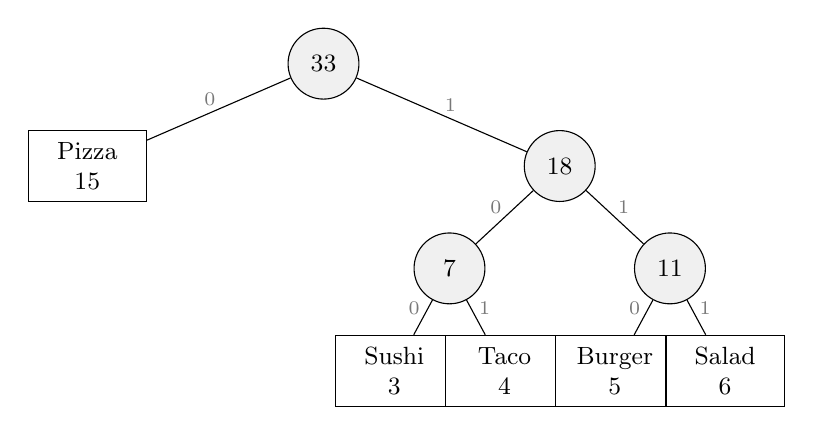
\begin{tikzpicture}[level distance=13mm,
  level 1/.style={sibling distance=60mm},
  level 2/.style={sibling distance=28mm},
  level 3/.style={sibling distance=14mm}]
\node[internal] {33}
  child { node[leaf] {Pizza\\ 15} edge from parent node[edgelabel,above left]{0} }
  child { node[internal] {18}
    child { node[internal] {7}
      child { node[leaf] {Sushi\\ 3} edge from parent node[edgelabel,above left]{0} }
      child { node[leaf] {Taco\\ 4}  edge from parent node[edgelabel,above right]{1} }
      edge from parent node[edgelabel,above left]{0}
    }
    child { node[internal] {11}
      child { node[leaf] {Burger\\ 5} edge from parent node[edgelabel,above left]{0} }
      child { node[leaf] {Salad\\ 6}  edge from parent node[edgelabel,above right]{1} }
      edge from parent node[edgelabel,above right]{1}
    }
    edge from parent node[edgelabel,above right]{1}
  };
\end{tikzpicture}
\vfill
\hintline{Depth multiset $\{1,3,3,3,3\}$. Two mini-trees sitting side by side under the 18.}
\end{frame}

% ======================================================================
\begin{frame}{Codes \& savings}
\vfill
\centering
\renewcommand{\arraystretch}{1.2}
\begin{tabular}{lcccc}
\toprule
Symbol & Count & Code & Length & Bits \\
\midrule
Pizza  & 15 & \texttt{0}   & 1 & 15 \\
Sushi  & 3  & \texttt{100} & 3 & 9  \\
Taco   & 4  & \texttt{101} & 3 & 12 \\
Burger & 5  & \texttt{110} & 3 & 15 \\
Salad  & 6  & \texttt{111} & 3 & 18 \\
\midrule
       &    &              &   & \ans{69} \\
\bottomrule
\end{tabular}
\vfill
\begin{center}\large
Huffman: \ans{69 bits}. \quad Naive: 99 bits. \quad Saved: \ans{30\%}.
\end{center}
\vfill
\hintline{Pizza is half the data, so Pizza gets one bit. The other four each get three.}
\end{frame}

% ======================================================================
% EXAMPLE 2 --- WEATHER LOG
% ======================================================================
\begin{frame}{\Large Example 2 --- Weather Log (more dramatic)}
\vfill
\begin{center}
\large ``Meteorologist's log, 62 hours. Sunny dominates; four wet conditions are rare and roughly equal.''
\end{center}
\vfill
\begin{columns}[T]
\column{0.45\textwidth}
\centering
\renewcommand{\arraystretch}{1.15}
\begin{tabular}{lc}
\toprule
State   & Count \\
\midrule
Sunny   & 32 \\
Cloudy  & 12 \\
Rainy   & 6  \\
Drizzle & 5  \\
Snow    & 4  \\
Hail    & 3  \\
\midrule
Total   & 62 \\
\bottomrule
\end{tabular}

\column{0.55\textwidth}
\small
\textbf{Five merges}
\begin{enumerate}
  \item Hail$(3)$ + Snow$(4) = 7$
  \item Drizzle$(5)$ + Rainy$(6) = 11$
  \item $7 + 11 = 18$
  \item Cloudy$(12) + 18 = 30$
  \item Sunny$(32) + 30 = 62$
\end{enumerate}
\vspace{0.5em}
Naive: $3 \times 62 = \ans{186 \text{ bits}}$.
\end{columns}
\end{frame}

% ======================================================================
\begin{frame}{Weather --- tree \& codes}
\begin{columns}[T]
\column{0.55\textwidth}
\centering
\vspace{0.5em}
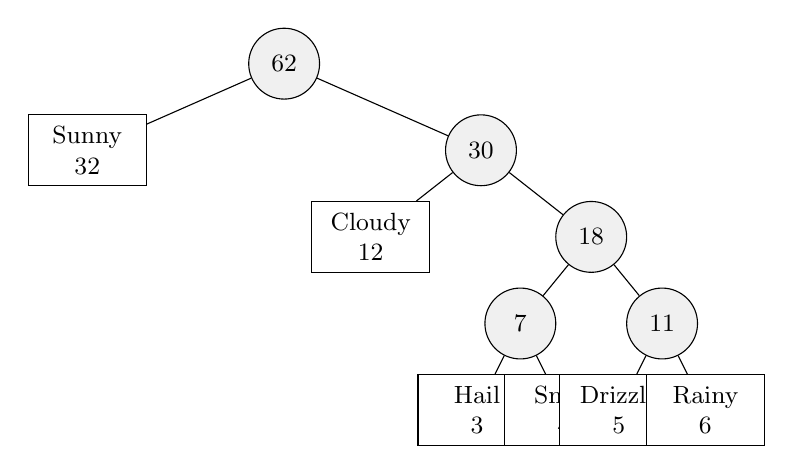
\begin{tikzpicture}[level distance=11mm,
  level 1/.style={sibling distance=50mm},
  level 2/.style={sibling distance=28mm},
  level 3/.style={sibling distance=18mm},
  level 4/.style={sibling distance=11mm}]
\node[internal] {62}
  child { node[leaf] {Sunny\\ 32} }
  child { node[internal] {30}
    child { node[leaf] {Cloudy\\ 12} }
    child { node[internal] {18}
      child { node[internal] {7}
        child { node[leaf] {Hail\\ 3} }
        child { node[leaf] {Snow\\ 4} }
      }
      child { node[internal] {11}
        child { node[leaf] {Drizzle\\ 5} }
        child { node[leaf] {Rainy\\ 6}  }
      }
    }
  };
\end{tikzpicture}

\column{0.45\textwidth}
\small
\renewcommand{\arraystretch}{1.15}
\begin{tabular}{lccc}
\toprule
Symbol  & Code & Len & Bits \\
\midrule
Sunny   & \texttt{0}    & 1 & 32 \\
Cloudy  & \texttt{10}   & 2 & 24 \\
Hail    & \texttt{1100} & 4 & 12 \\
Snow    & \texttt{1101} & 4 & 16 \\
Drizzle & \texttt{1110} & 4 & 20 \\
Rainy   & \texttt{1111} & 4 & 24 \\
\midrule
        &               &   & \ans{128} \\
\bottomrule
\end{tabular}
\vspace{0.5em}

186 $\to$ \ans{128} bits. Saved \ans{31\%}.\\
Depth shape $\{1,2,4,4,4,4\}$.
\end{columns}
\vfill
\hintline{Three distinct code lengths. Sunny is half the log; the four wet states are each rare \emph{and comparable}, so they share a code length.}
\end{frame}

% ======================================================================
% EXAMPLE 3 --- DESSERT MENU
% ======================================================================
\begin{frame}{\Large Example 3 --- Dessert Menu (no dominant symbol)}
\vfill
\begin{center}
\large ``22 desserts, five kinds. No runaway favorite. Can Huffman still find structure?''
\end{center}
\vfill
\begin{columns}[T]
\column{0.45\textwidth}
\centering
\renewcommand{\arraystretch}{1.15}
\begin{tabular}{lc}
\toprule
Kind    & Count \\
\midrule
Cake    & 7 \\
Brownie & 6 \\
Cookie  & 5 \\
Pie     & 3 \\
Tart    & 1 \\
\midrule
Total   & 22 \\
\bottomrule
\end{tabular}

\column{0.55\textwidth}
\small
\textbf{Four merges}
\begin{enumerate}
  \item Tart$(1)$ + Pie$(3) = 4$
  \item $4$ + Cookie$(5) = 9$
  \item Brownie$(6)$ + Cake$(7) = 13$ \textcolor{accent}{\textit{(separate pile!)}}
  \item $9 + 13 = 22$
\end{enumerate}
\vspace{0.5em}
Naive: $3 \times 22 = \ans{66 \text{ bits}}$.
\end{columns}
\end{frame}

% ======================================================================
\begin{frame}{Dessert --- tree \& codes}
\begin{columns}[T]
\column{0.55\textwidth}
\centering
\vspace{0.5em}
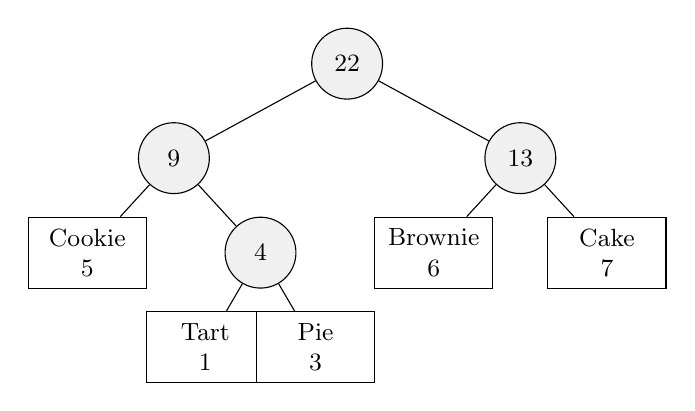
\begin{tikzpicture}[level distance=12mm,
  level 1/.style={sibling distance=44mm},
  level 2/.style={sibling distance=22mm},
  level 3/.style={sibling distance=14mm}]
\node[internal] {22}
  child { node[internal] {9}
    child { node[leaf] {Cookie\\ 5} }
    child { node[internal] {4}
      child { node[leaf] {Tart\\ 1} }
      child { node[leaf] {Pie\\ 3}  }
    }
  }
  child { node[internal] {13}
    child { node[leaf] {Brownie\\ 6} }
    child { node[leaf] {Cake\\ 7}    }
  };
\end{tikzpicture}

\column{0.45\textwidth}
\small
\renewcommand{\arraystretch}{1.2}
\begin{tabular}{lccc}
\toprule
Symbol  & Code & Len & Bits \\
\midrule
Cookie  & \texttt{00}  & 2 & 10 \\
Brownie & \texttt{10}  & 2 & 12 \\
Cake    & \texttt{11}  & 2 & 14 \\
Tart    & \texttt{010} & 3 & 3  \\
Pie     & \texttt{011} & 3 & 9  \\
\midrule
        &              &   & \ans{48} \\
\bottomrule
\end{tabular}
\vspace{0.5em}

66 $\to$ \ans{48} bits. Saved \ans{27\%}.\\
Depth shape $\{2,2,2,3,3\}$.
\end{columns}
\vfill
\hintline{Root splits into \emph{two} internal nodes. Most symmetric of the three trees --- even when no symbol dominates, Huffman still beats the naive code.}
\end{frame}

% ======================================================================
% SYNTHESIS
% ======================================================================
\begin{frame}{What the three trees share}
\large
\begin{itemize}
  \item All three trees \emph{branch} at some internal level --- neither child of the root (or the child of that child) is the lone spine.
  \item Integer counts chosen so every merge value is distinct from every other pile --- \textbf{no tie-breaking pauses}.
  \item Frequent symbols end up with short codes; rare ones with long codes.
  \item 27--31\% savings vs the naive 3-bit code --- without any prior agreement between encoder and decoder.
\end{itemize}
\vfill
\begin{center}
\small\textcolor{hint}{Depth shapes: $\{1,3,3,3,3\}$, \ $\{1,2,4,4,4,4\}$, \ $\{2,2,2,3,3\}$.}
\end{center}
\end{frame}

% ======================================================================
\begin{frame}{Why we care}
\vfill
\begin{itemize}
  \item Huffman trades \textbf{known frequencies} for \textbf{shorter codes}.
  \item Knowing frequencies $=$ having a \textbf{probabilistic model} of the source.
  \item The better your model, the shorter the expected code. \\(Shannon: $L^* \approx H(X)$.)
\end{itemize}
\vfill
\begin{center}
\Large \textbf{good prediction $\;\Longleftrightarrow\;$ good compression}
\end{center}
\vfill
\begin{center}
\small\textcolor{hint}{A language model that predicts the next token well compresses the training corpus. That's the thread from Shannon $\to$ Solomonoff $\to$ Kolmogorov $\to$ modern LLMs.}
\end{center}
\end{frame}

% ======================================================================
% INSTRUCTOR PICKING GUIDE
% ======================================================================
\begin{frame}{Instructor reference --- which example to pick}
\small
\renewcommand{\arraystretch}{1.4}
\begin{tabular}{l p{2.3cm} p{2.0cm} p{4.7cm}}
\toprule
Example & Depth shape & Savings & Pick when\ldots \\
\midrule
Lunch Menu    & $\{1,3,3,3,3\}$   & 30.3\% & Default. Cleanest board, sharpest story, clearest ``two piles side by side.'' \\
Weather Log   & $\{1,2,4,4,4,4\}$ & 31.2\% & Audience is comfortable with arithmetic and you want the widest depth range (1 to 4) and three code-length tiers. \\
Dessert Menu  & $\{2,2,2,3,3\}$   & 27.3\% & No dominant symbol --- show that Huffman still finds structure. Smallest numbers on the board (all $\le 7$). \\
\bottomrule
\end{tabular}
\vfill
\hintline{All three: bushy, tie-free merges, $\le$~5 min with slack, no information-theory background required.}
\end{frame}

\end{document}
